\documentclass[10pt,a4paper, titlepage]{report}

\usepackage[utf8]{inputenc}
\usepackage[czech]{babel}

\usepackage{titlesec, blindtext, color}
\definecolor{gray75}{gray}{0.75}
\newcommand{\hsp}{\hspace{20pt}}
\titleformat{\chapter}[hang]{\Huge\bfseries}{\thechapter\hsp\textcolor{gray75}{|}\hsp}{0pt}{\Huge\bfseries}

\usepackage[T1]{fontenc}
\usepackage{amsmath}
\usepackage{amsfonts}
\usepackage{amssymb}
\usepackage{graphicx}
\usepackage{verbatim}
\usepackage{a4wide}
\usepackage{verbatim}
\newenvironment{mylisting}
{\begin{list}{}{\setlength{\leftmargin}{1em}}\item\scriptsize\bfseries}
{\end{list}}

\begin{document}
\begin{titlepage}
\begin{center}

% Upper part of the page. The '~' is needed because \\
% only works if a paragraph has started.


\includegraphics[width=0.3\textwidth]{pics/logo_cvut.jpg}\\[0.4cm]

\textsc{České vysoké učení technické v Praze\\Fakulta stavební}\\[0.4cm]
\textsc{\\\small{Projekt Informatika 2} \\\small{Akedemický rok 2012/2013}}\\[0.4cm]

% Title
 \huge \bfseries{Mapa kamer -- mobilní aplikace pro Android}\\\textsc{\small{Dokumentace}}\\[0.4cm]

% Author and supervisor
\begin{minipage}{0.4\textwidth}
\begin{flushleft} \large
\emph{Autoři:}\\
Martin \textsc{Lžíčař}\\
Dan \textsc{Dluhoš}\\ 
Michal \textsc{Med}
\end{flushleft}
\end{minipage}
\begin{minipage}{0.4\textwidth}
\begin{flushright} \large
\emph{Vedoucí:} \\
Ing. Martin \textsc{Landa}\\
Katedra mapování a kartografie\\
K153
\end{flushright}
\end{minipage}

\vfill


\end{center}
\end{titlepage}

\tableofcontents
\newpage

\chapter*{Zadání}
\verbatiminput{sections/zadani.txt}

\chapter{Úvod}
Práce byla vytvořena v rámci projektu informatika 2 ve spolupráci s občanským sdružením IuRe -- Iuridicum Remedium. Sdružení se zabývá ochranou soukromí a lidskými právy. Na svých stránkách\footnote{www.iure.org} zveřejňují mimo jiné \uv{výherce} ankety \texttt{Big brother awards} nebo webovou aplikaci mapa kamer\footnote{www.mapakamer.cz}, ve které zobrazují veřejná místa pokrytá kamerovými systémy. 
\begin{figure}[hb]
\begin{center}

\includegraphics[scale=0.3]{pics/iure_logo.png}
\caption{Logo občanského sdružení IuRe}
\end{center}
\end{figure}
\begin{figure}[hb]
\begin{center}
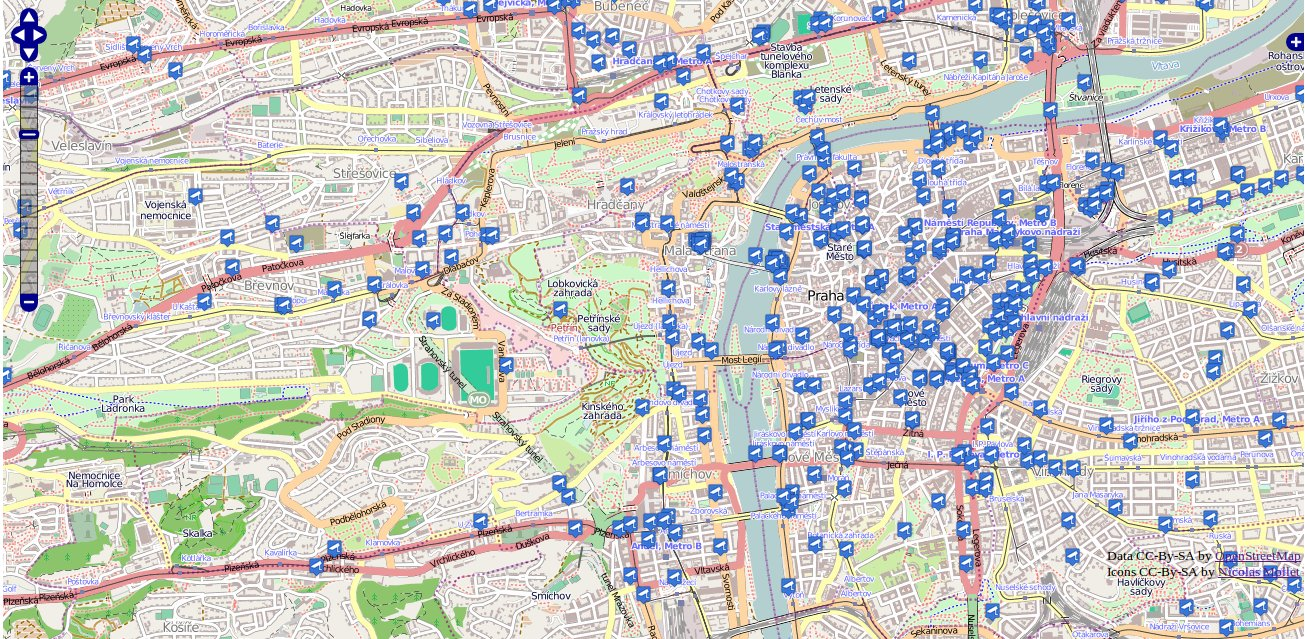
\includegraphics[scale=0.3]{pics/mapakamer.jpg}
\caption{Webová aplikace Mapa kamer}
\end{center}
\end{figure}
\paragraph{}
Sdružení se již v minulosti pokoušelo o tvorbu mobilní aplikace pro zaznámenávání a zobrazování kamer, ale potýkalo se s nedostatkem pracovních kapacit, proto naši bezplatnou nabídku ke spolupráci rádi přijali. Základ aplikace byl již připraven, ale nespl\v{n}oval ani jejich ani naše očekávání. Aplikace byla založena na \texttt{Google Maps} a neměla v pozadí ani databázi, ani server. I o to jsme se tedy museli postarat. 
\paragraph{}
Aplikace je zacílena na mobilní operační systém \texttt{Android}. Jazykem běžně používaným pro tvorbu aplikací pro \texttt{Android} je \texttt{Java}. Použili jsme vývojové prostředí \texttt{Eclipse}, do kterého je však pro tvorbu mobilních aplikací potřeba doinstalovat \texttt{Android Developer Tools}.
\begin{figure}[hb]
\begin{center}

\includegraphics[scale=0.1]{pics/android.jpg}
\end{center}
\end{figure} 
\paragraph{}
Jako podkladová mapa byly použity rastry z opensourcového projektu \texttt{OpenStreetMap}\footnote{www.openstreetmap.org}. Pro uchovávání informací o kamerách byla použita databáze \texttt{PostgreSQL} a dále byla, opět v jazyce \texttt{Java}, napsána webová aplikace umož\v{n}ující komunikaci mezi mobilním zařízením a databází.
\newpage

\chapter{Mobilní aplikace Mapa Kamer}
Tato kapitola se zabývá tvorbou a používáním mobilní aplikace. V jednotlivých sekcích se zmíníme o přípravě prostředí \texttt{Eclipse} pro vývoj mobilních aplikací pro systém \texttt{Android}, s používáním projektu \texttt{Osmdroid}\footnote{http://code.google.com/p/osmdroid/}, který slouží k používání map projektu \texttt{OpenStreetMap} v \texttt{Androidu} a o tom, jak do databáze přidat novou kameru. Na závěr kapitoly se zmíníme o specifikách vývoje aplikací pro systém \texttt{Android} jako takových.
\section{Příprava prostředí Eclipse pro vývoj Android aplikací}
Balíček \texttt{ADT Bundle} poskytuje vše, co je potřeba k vývoji aplikací pro Android, včetně \texttt{Eclipse IDE} s vestavěným ADT (\texttt{Android Developer Tools}). Je možné nainstalovat \texttt{Android STK} i do existujícího IDE\footnote{http://developer.android.com/sdk/installing/index.html}, ale zde se budeme zabývat instalací celého balíčku \texttt{ADT Bundle}.
\paragraph{}
Po rozbalení do zvoleného adresáře stačí otevřít adresář adt-bundle-<os\_platform>/eclipse/ a spustit z něj \texttt{eclipse}. IDE je rovnou načteno s pluginem \texttt{ADT} a SDK je připraveno k použití.
\begin{figure}[hb]
\begin{center}
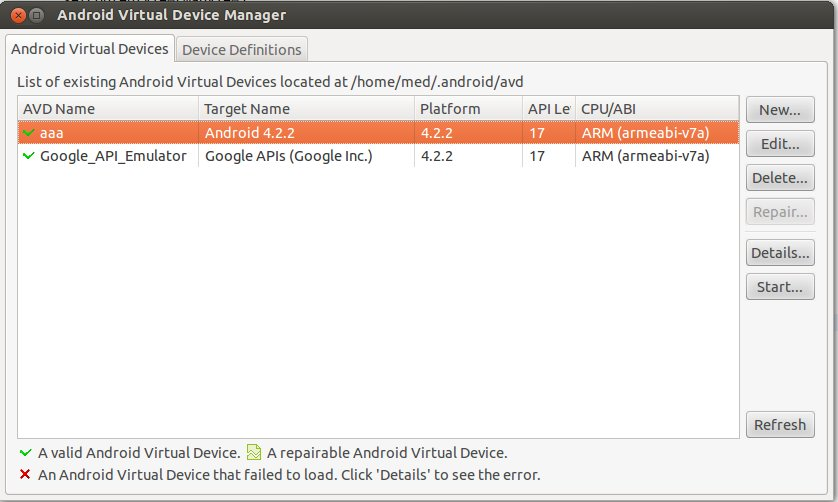
\includegraphics[scale=0.4]{pics/emulator_nastaveni.jpg}
\caption{Správně nastavený emulátoru je na druhém řádku}
\end{center}
\end{figure}
\paragraph{}
Balíček obsahuje vše nezbytné včetně emulátoru. Ke správě, spuštění a nastavení SDK slouží položka v menu \textbf{Window} $\rightarrow$ \textbf{Android SDK Manager}, ke správě emulátoru potom \textbf{Window} $\rightarrow$ \textbf{Android Virtual Device Manager}. K bezproblémovému chodu aplikace v emulátoru je potřeba nastavit jako cílové prostředí \texttt{Google APIs} v poslední verzi (17).
\paragraph{}
Nejnovější verze \texttt{Google API} v nabídce pravděpodobně nebude. K její instalaci je třeba otevřít \textbf{Window} $\rightarrow$ \textbf{Android SDK Manager} a doinstalovat ho. 
\begin{figure}[hb]
\begin{center}
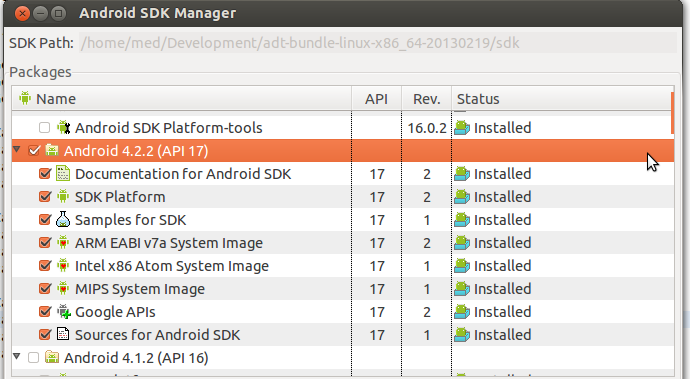
\includegraphics[scale=0.5]{pics/SDK_manager.png}
\caption{Označené balíčky je potřeba doinstalovat}
\end{center}
\end{figure}
\paragraph{}
Pro spuštění aplikace \texttt{Mapa Kamer} v emulátoru je potřeba ještě nastavit souřadnice GPS. To se musí udělat ručně, protože emulátor nemá žádné fyzické GPS zařízení. ze to udělat dvěma způsoby:
\begin{itemize}
\item Ruční nastavení v DDMS:
\begin{itemize}
\item \textbf{Window} $\rightarrow$ \textbf{Open Perspective} $\rightarrow$ \textbf{DDMS},
\item označit emulátor a v záložce \textbf{Emulator Control} nastavit souřadnice,
\item potvrdit tlačítkem \textbf{Send}.
\end{itemize}
\begin{figure}[hb]
\begin{center}
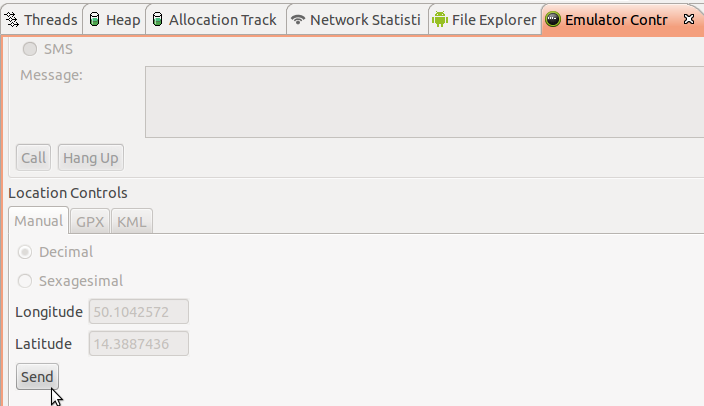
\includegraphics[scale=0.3]{pics/ddms.png}
\caption{Označené balíčky je potřeba doinstalovat}
\end{center}
\end{figure}
\item Pomocí telnetu:
\begin{itemize}
\item otevřít konzoli,
\item připojit zařízení: \texttt{telnet localhost 5554},
\item nastavit souřadnice: \texttt{geo fix 13.24 52.31}.
\end{itemize}
\end{itemize}
Je celkem jedno který z těchto způsobů je použit. Po správném nastavení souřadnic by se měl emulátor chovat jako mobilní zařízení v poloze nastavené těmito souřadnicemi. \textbf{Pozor}: nastavením GPS souřadnic není v zařízení "zapnut" GPS modul. GPS se zapíná v nastavení (\textbf{Menu} $\rightarrow$ \textbf{Settings} $\rightarrow$ \textbf{Location access} $\rightarrow$ \textbf{GPS satellites}). 

\section{Projekt Osmdroid}
V \texttt{Android SDK} existuje mapová podpora pro \texttt{Google Maps}, protože \texttt{Android} patří také společnosti \texttt{Google}. Pro použití \texttt{OpenStreetMap} v aplikaci existuje více možností, kromě námi použitého \texttt{Osmdroid} lze použít například renderovací knihovnu \texttt{MapsForge}\footnote{http://code.google.com/p/mapsforge/}.
\paragraph{}
Balíček \texttt{Osmdroid} umožňuje používání nativních metod pro zobrazování \texttt{Google Maps} k zobrazování dat z projektu \texttt{OpenStreetMap}. V některých případech, jako je třeba zobrazení mapy, její vycentrování nebo nastavení hladiny zoom, se používají metody knihovny \texttt{Osmdroid} přesně jako ekvivalentní metody z balíčku \texttt{google.maps}. V některých jiných případech jsou třídy poněkud odlišné. Příkladem může být třeba zobrazení markerů (třída \texttt{ItemizedOverlay}). V některých případech nám možnosti hotových tříd nestačily a požadovanou funkčnost jsme museli dopsat sami. Stalo se nám to například u zobrazení obrázku v informačním okně vyskakujícím při poklepání na marker v mapě. Pro tento účel jsme vytvořili třídu \texttt{ImageOverlayItem}.
\paragraph{}
Od používání \texttt{OpenStreetMap} na úkor \texttt{Google Maps} jsme si slibovali možnost využití vrstvy \texttt{surveillance} z databáze \texttt{OpenStreetMap}, která obsahuje poměrně velké množství kamer sledujících veřejný prostor a která byla použita ve webové aplikaci Mapa Kamer a z velké míry i dopl\v{n}ována díky aktivitám sdružení  IuRe. K zobrazování vrstvy jsou ve webové aplikaci použity \texttt{OpenLayers}, které ale neexistují ve verzi pro mobilní zařízení, jedině v prohlížeči. Pokoušeli jsme se nalézt nějaké řešení jak použít data z této vrstvy a nakonec jsme se rozhodli pro export dat z databáze \texttt{OpenStreetMap} do lokální databáze na našem serveru. Odtud je možné data normálně zobrazovat v mobilní aplikaci.

\section{Používání aplikace}
Při spuštění aplikace má uživatel na výběr mezi třemi tlačítky:
\begin{itemize}
\item Přidat kameru,
\item Zobrazit mapu kamer,
\item O projektu.
\end{itemize}

\subsection{Přidat kameru}
Nové kamery jsou přidávány přímo do databáze na serveru. Tato databáze se synchronizuje přímo s databází \texttt{OpenStreetMap}. O databázi i samotném nahrávání nové kamery po technické stránce se zmíníme ještě v dalších kapitolách. V této sekci popíšeme co a jak dělat v aplikaci aby byla nová kamera odeslána.
\begin{figure}[!ht]
\begin{center}

\includegraphics[scale=0.2]{pics/open_GPS.jpg}
\caption{Dialog vybízející k zapnutí GPS}
\end{center}
\end{figure}
\paragraph{}
Při otevření aktivity  aplikace nejprve zkontroluje, zda je zapnutá GPS. Pokud ne, dostane uživatel možnost GPS zapnout a zlepšit tak přesnost zaměření polohy.
\paragraph{} Pokud GPS nezapne, bude poloha určena ze sítě. Poloha je zobrazena na řádku \texttt{GPS lokace}. Do řádku \texttt{popis kamery} uživatel napíše něco o kameře. Mělo by se to týkat faktických věcí, jako například kdo je provozovatelem kamery, upřesnění její polohy nebo například to, jestli kamera pouze zobrazuje, nebo i nahrává záznam. Poslední věc kterou je ke kameře možné přidat je fotografie. Po stisknutí tlačítka je uživatel přesměrován do aplikace fotoaparátu, kterou pořídí snímek. Poté už stačí celý formulář jenom potvrdit a kamera bude přidána do databáze.

\subsection{Zobrazit mapu kamer}
Při spuštění mapy aplikace nejprve zkontroluje, zda je zapnutá GPS. V případě že ano, je na aktuálních souřadnicích vycentrována mapa \texttt{OpenStreetMap}. Pokud GPS zapnutá není, zobrazí se stejný dialog jako v předchozí sekci a uživatel dostane možnost zapnout GPS.
\paragraph{}
Při volbě \textbf{Ano} je uživatel přesměrován do nastavení správy GPS. GPS může, ale nemusí být zapnutá. Pro určení polohy z GPS je použit objekt \texttt{gpsLocListener}. V případě, že se uživatel rozhodne nechat GPS vypnutou (a zvolí \textbf{Ne}), je poloha určována ze sítě pomocí objektu \texttt{networkLocListener}. 
\begin{figure}[!ht]
\begin{center}
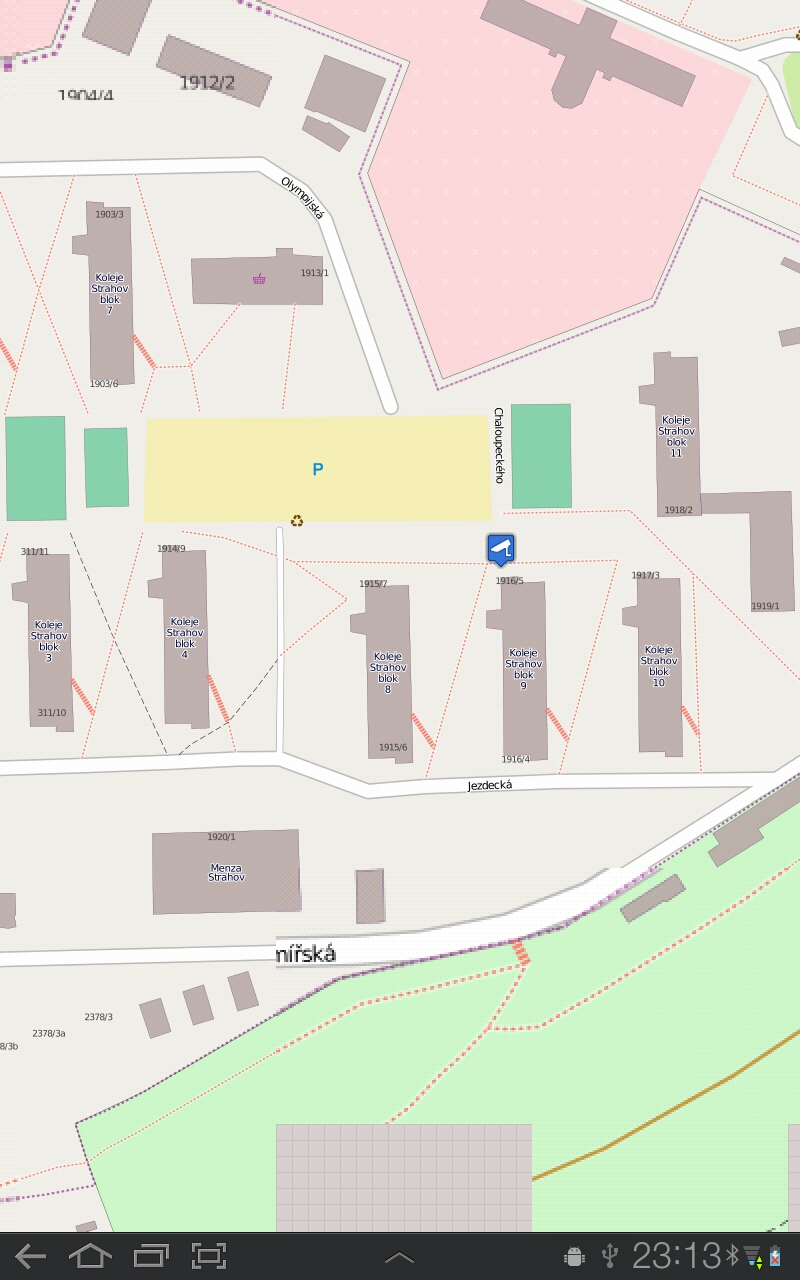
\includegraphics[scale=0.07]{pics/mapa.jpg}
\caption{Mapa vycentrovaná na místě, na kterém jsem psal tuto dokumentaci}
\end{center}
\end{figure}
\paragraph{}
Podklad \texttt{OpenStreetMap} je zobrazen a vycentrován na aktuální pozici. Z databáze jsou poté pomocí příkazu \texttt{SELECT} vytaženy kamery a zobrazeny s markerem se symbolem cctv\footnote{http://mapicons.nicolasmollet.com/markers/offices/cctv/}. Při poklepání na kameru se otevře informační okno s podrobnostmi o kameře. Kromě popisu může obsahovat i fotografii.
\begin{figure}[!ht]
\begin{center}
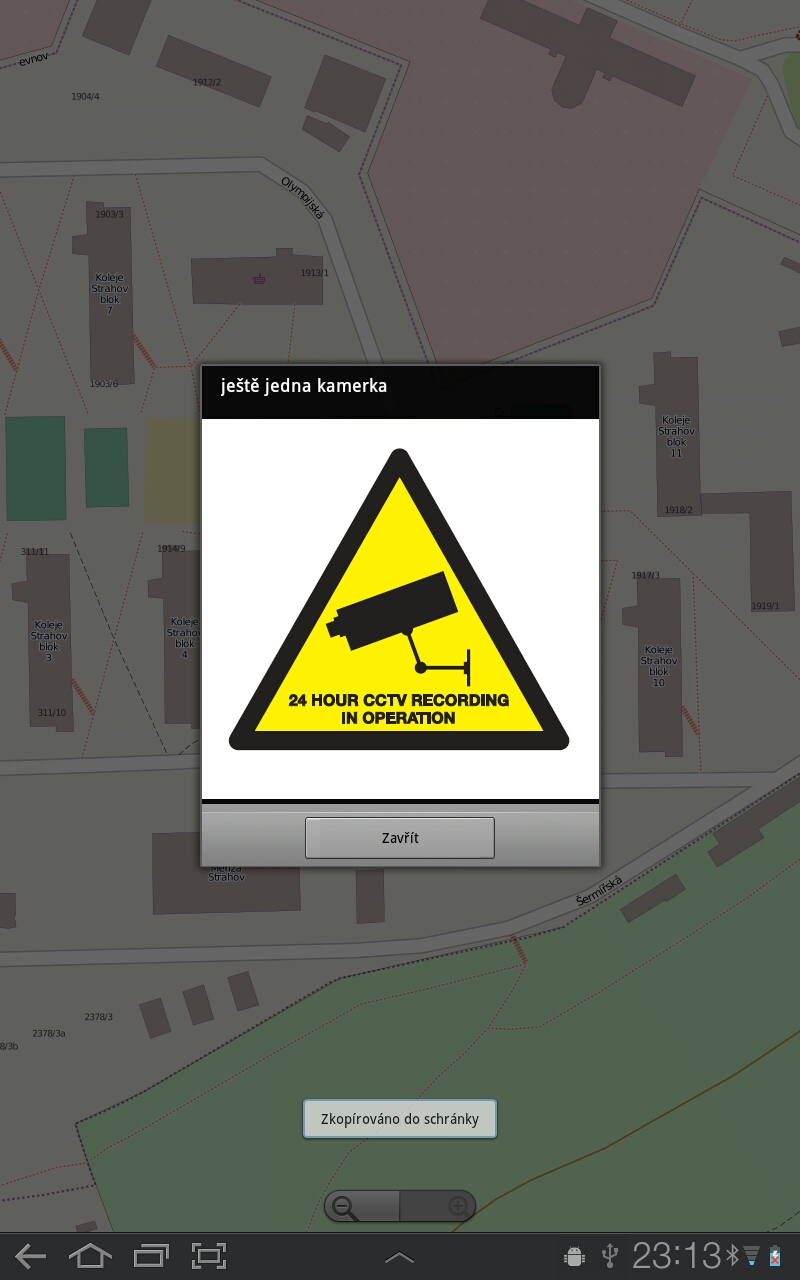
\includegraphics[scale=0.07]{pics/infoWindow.jpg}
\caption{Ukázka informačního okna kamery}
\end{center}
\end{figure}

\subsection{O projektu}
V této záložce se uživatel může dočíst jaké cíle má projekt Mapa kamer, na jakých principech je postaven a také něco o sdružení IuRe a tvůrcích projektu.
\begin{figure}[!ht]
\begin{center}
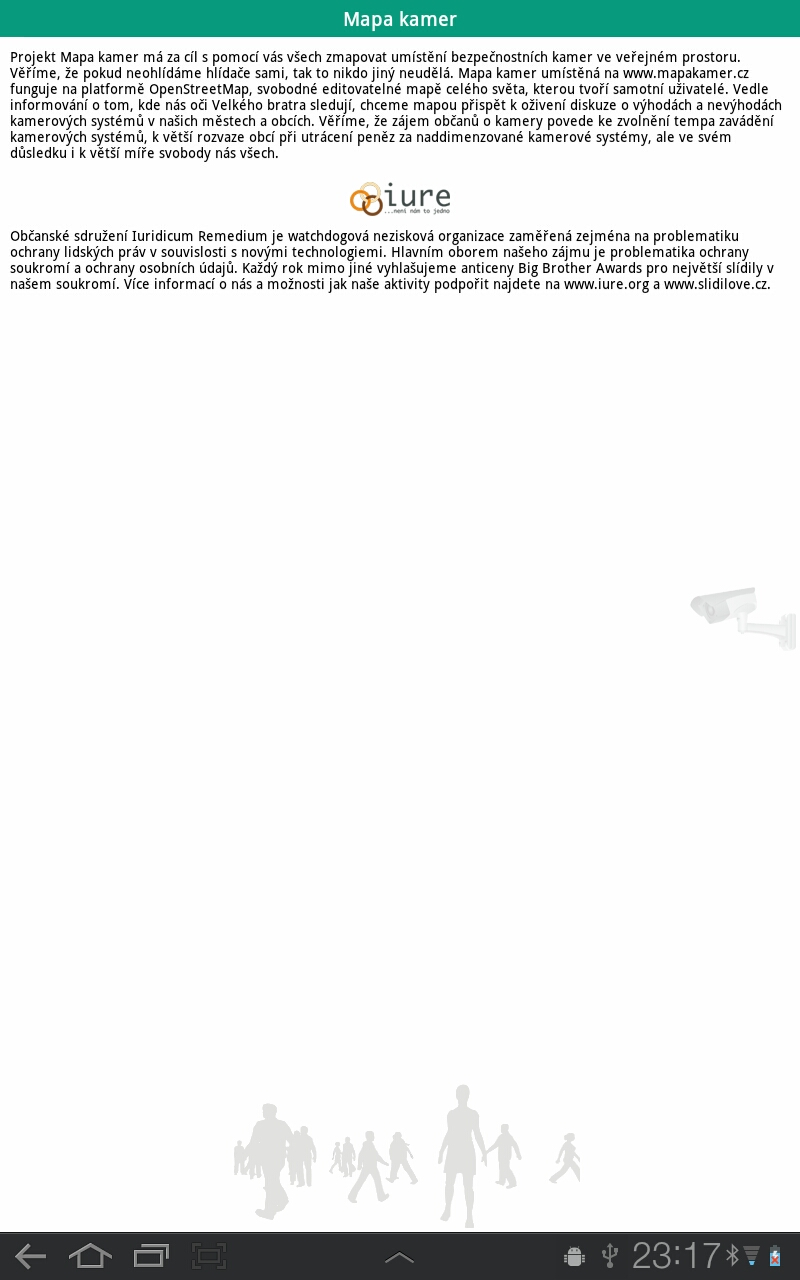
\includegraphics[scale=0.07]{pics/about.jpg}
\caption{Vzhled záložky O projektu (screenshot z tabletu)}
\end{center}
\end{figure}

\section{Základy vývoje aplikací pro Android}
Tvorba aplikace pro systém \texttt{Android} je ve své podstatě hrozně jednoduchá. Každá aplikace má jeden xml soubor pojmenovaný \texttt{Manifest}. Ten obsahuje název balíčku, verze systému pro které je aplikace určená a dále velmi důležitý seznam použitých povolení (\texttt{permissions}) a vlastností (\texttt{features}). Další věci jsou obsaženy v elementu application. Jedná se především o seznam aktivit používaných v aplikaci. Co je to aktivita je vysvětleno dále.
\paragraph{}
Aktivitu si lze představit jako jednu obrazovku mobilního zařízení s tlačítky, nadpisy, menu a vším co k tomu patří. V aplikaci Mapa Kamer je například jednou z aktivit \texttt{HomeActivity}, která obsahuje domácí obrazovku aplikace se třemi tlačítky. Při poklepání na tlačítka se akorát spouští další aktivity, jmenovitě to jsou \texttt{NewCameraActivity}, \texttt{CameraMapActivity} a \texttt{AboutActivity}. 
\begin{figure}[!ht]
\begin{center}
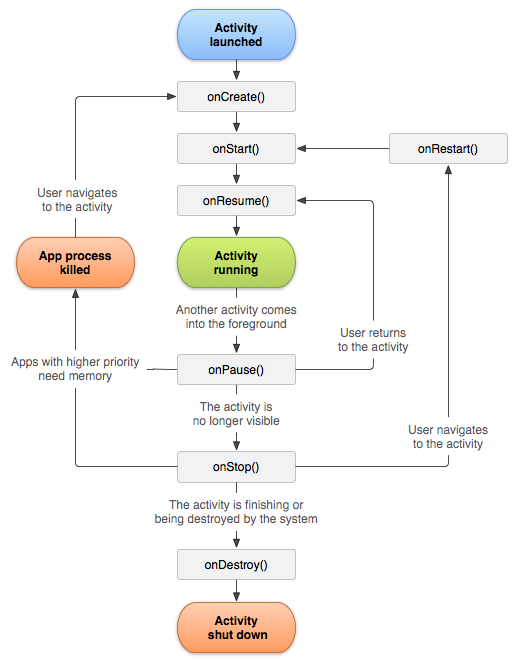
\includegraphics[scale=0.3]{pics/activity_lifecycle.png}
\caption{Životní cyklus aktivity}
\end{center}
\end{figure}
\paragraph{}
Každá aktivita může mít vzhled tvořen buď kódem v jazyce \texttt{Java}, nebo je možné vzhled nastavit pomocí xml souboru v \texttt{res} $\rightarrow$ \texttt{layout}. V prostředí \texttt{Eclipse} je možné xml vytvářet pomocí grafického editoru. 
\paragraph{}
Každá aktivita má svůj životní cyklus. Aktivita může být v jednom ze čtyř základních stavů:
\begin{itemize}
\item \textbf{Aktivní} -- aktivita běží v popředí.
\item \textbf{Pozastavená} -- aktivita je pořád viditelná, ale není aktivní. Chová se stejně jako aktivní aplikace, ale v případě malé paměti zařízení jí systém může zabít.
\item \textbf{Zastavená} -- aktivita je kompletně překryta jinou aktivitou. Když je paměť potřeba jinde, tak jí systém zpravidla zabije.
\item \textbf{Zabitá} -- pokud je pozastavená nebo zastavená aktivita zabita systémem a uživatel ji chce zobrazit, musí být znovu načtena úplně od začátku a uvedena zpět do předchozího stavu.
\end{itemize}
\paragraph{}
Každá aktivita má několik metod, kterými je možné ji uvést do některého z uvedených stavů. Metoda uvádějící aktivitu do určitého stavu má párovou metodu, která tento stav ukončí.
\begin{itemize}
\item \texttt{onCreate} a \texttt{onDestroy}
\item \texttt{onStart} a \texttt{onStop}
\item \texttt{onResume} a \texttt{onPaused}
\end{itemize}
\newpage

\chapter{Databáze}
Jako databáze na které aplikace pojede byla zvolena databáze \texttt{PostgreSQL}. Důvody jsou dva:
\begin{itemize}
\item Jedná se o open source projekt.
\item Projekt \texttt{OpenStreetMap} používá jako databázi také \texttt{PostgreSQL}.
\end{itemize}
\begin{figure}[!ht]
\begin{center}

\includegraphics[scale=0.5]{pics/postgresql_logo.png}
\caption{Logo projektu PostgreSQL, na kterém slon reprezentuje dobrou pamě\v{t}}
\end{center}
\end{figure}
\paragraph{}
Základem pro databázi bylo schéma, které nám laskavě poskytl pan inženýr Martin \textsc{Landa}. Schéma obsahovalo data \texttt{OpenStreetMap} pro Českou Republiku. Ze schématu jsme vytáhli pomocí následujícího příkazu vytáhli všechny body s tagem \textbf{surveillance} a uložili je do tabulky \texttt{b\_kamery}.
\paragraph{}
\texttt{CREATE TABLE b\_kamery AS (SELECT osm\_id,name,ST\_X(ST\_Transform(way::geometry,4326)) AS lat,ST\_Y(ST\_Transform(way::geometry,4326)) AS lon FROM osm.czech\_point WHERE man\_made ='surveillance');}
\paragraph{}
Tabulka \texttt{b\_kamery} obsahuje identifikátor, informace o kameře, souřadnice kamery, které byly naimportovány ze schématu \texttt{osm} a navíc jsme přidali atribut \texttt{image}, který zatím obsahuje adresu obrázku na serveru. Do budoucna plánujeme obrázky ukládat jako BLOB\footnote{Binary Large OBject}, protože při větším množství obrázků by pravděpodobně byl velký problém s pamětí. Z důvodů nevhodného k\'{o}dování se v informačním okně kamery zobrazuje pouze obrázek a nikoliv popis kamery.
\paragraph{}
Pro zrychlení vyhledávacích a dotazovacích procesů v databázi bude záhodno databázi naindexovat. Indexy v databázi by ji mohli výrazně zrychlit a zvláště u pomalejších zařízeních a zařízeních s menší kapacitou paměti to dost pomůže rychlému chodu aplikace. Principem indexování je přenesení paměťové a kapacitní náročnosti ze zařízení na server, což by při porovnání výpočetní kapacity serveru a výpočetní kapacity mobilního zařízení nemělo vůbec vadit. 
\newpage

\chapter{Připojení k databázi na serveru}
Kapitola se věnuje řešením a problémům při práci na propojení mobilní aplikace s databází. Naším požadavkem bylo načítat data z databáze a zároveň do ní data i vkládat. Zkusili jsme několik způsobů, které krátce popíšeme a poté se podrobněji zaměříme na řešení, které bylo zvoleno.

\paragraph{}
Jako první jsme vymysleli, že z mobilní aplikace by se poslal požadavek \texttt{http post} na \texttt{php} skript na serveru. Ten by pracoval s databází a prováděl požadované operace nad daty. Tento způsob se nám nepodařilo implementovat a dozvěděli jsme se, že to není bezpečný způsob. Proto jsme další vývoj přerušili a zkusili něco jiného.

\paragraph{}
Implementovali jsme možnost, že by se samotná mobilní aplikace připojila přímo do databáze. Tento způsob fungoval a oba naše požadavky byly splněny. Ale při hledání řešení jsme objevili, že tento způsob je velmi náročný na výpočetní techniku, protože navázání spojení je to nejtěžší na celém procesu připojení aplikace k databázi. Po konzultaci s doktorem Janem Pytlem jsme se rozhodli použít \texttt{Java Servlety}.

\section{Java Servlet}
Servlet je třída v jazyce Java, která rozšiřuje možnosti serveru. Servlet umí zpracovat požadavek \texttt{request} a odpovědět \texttt{response}. Musí běžet na serveru, který zvládne zpracovat programovací jazyk Java. Použili jsme \texttt{Apache Tomcat 7}\footnote{http://tomcat.apache.org/}. Ten implementuje verzi \texttt{Servlet 3.0}, jehož možnosti jsme využili a zmíníme je dále.
\paragraph{}
Webová aplikace se servlety si s použitím interfacu \texttt{DataSource} předpřipraví připojení do databáze a vyhne se tím problému náročného přímého přístupu do databáze. Tyto předpřipravené připojení pak \uv{půjčuje} servletům, které reagují na požadavky z mobilní aplikace. Nastavení připojení se nastavuje v souboru \texttt{context.xml}. V tomto souboru jsou přihlašovací údaje do databáze. K tomuto souboru má přístup pouze administrátor a jiná bezpečnostní opatření se zpravidla neaplikují\footnote{Konzultace s Ing. Janem Pytlem Ph.D.}.

\paragraph{}
Z důvodů popsaných výše jsme vytvořili jednoduchou webovou aplikaci obsahující následující dva servlety. 
\begin{itemize}
\item Servlet \textbf{GetFromDB.java}, který se stará o získávání dat z databáze. Podle parametru získaného z \texttt{HttpServletRequest} je nastavena odpověď do \texttt{HttpServletResponse}. Parametrem je adresa umístění obrázku, který bude následně odeslán do mobilního zařízení. Pokud není žádný parametr uveden, pak jsou do mobilní aplikace poslány všechny kamery z databáze.
\item Servlet \textbf{SaveToDB.java}, který z částí \texttt{HttpServletRequest} získá informace o nově přidávané kameře a vloží ji do databáze. V tomto servletu byly použity nové technologie z verze \texttt{Servletu 3.0}. Pří sestavování požadavku o kameře v mobilní aplikaci byl použit objekt \texttt{MultipartEntity}. Ten umož\v{n}uje poslat jedním http postem jak samotný text, tak i soubory, což jsou v našem případě fotografie kamer. Ty jsou ukládány v adresáři pod jmény podle času vložení. to zajiš\v{t}uje unikátní název souboru, který je uložen do databáze.
\end{itemize}

\section{Vytváření požadavku v mobilním zařízením}
Požadavek na server se vytváří v mobilním zařízením ve třech případech.
\begin{itemize}
\item \textbf{Poslání nové kamery do databáze} - pomocí výše zmíněné \texttt{MultipartEntity} se posílají všechna data (např. souřadnice, obrázek kamery) ke zpracovaní do webové aplikace.
\item \textbf{Při zobrazení mapy kamer} - neposílá se žádný parametr, ale z webové aplikace se získávají data o kamerách. V databázi není uložen přímo obrázek, ale pouze cesta na místo na serveru kde je obrázek uložen. Aplikace vytáhne soubor ze serveru a použije ho v informačním okně kamery jako její obrázek. V současné době se načítají z databáze všechny kamery, což je velmi náročné na pame\v{t} mobilního zařízení. V dalším vývoji aplikace se tento problém vyřeší nahráním kamer pouze z okolí současné lokace přístroje.
\item \textbf{Při zobrazení obrázku kamery} - jako parametr se nastavuje název souboru s obrázkem kamery, na kterou uživatel poklepal. Tento obrázek se zobrazí na obrazovce mobilního zařízení. 
\end{itemize} 
Při vytváření požadavků na server jsme narazili na zajímavý problém. Pokud byl požadavek vytvářen přímo v dané aktivitě, tak tento požadavek nešel poslat na server. Důvod byl ten, že od určité verze Android API nešel poslat požadavek v hlavním vlákně aplikace. Pomocí třídy \texttt{AsyncTask} \footnote{http://developer.android.com/reference/android/os/AsyncTask.html} lze jednoduše provádět operace v jiném vlákně aplikace, ve kterém se provede odeslání požadavku na server. 
\newpage

\chapter{Problémy při implementaci aplikace}
S problémy jsme se setkávali téměř nepřetržitě. Verze, kterou teď prezentujeme, se od verze kterou odevzdáme sdružení IuRe ještě trochu liší právě proto, že jsme se některé z problémů zatím rozhodli ignorovat (pokud přímo nenarušují chod aplikace) a vyřešíme je před odevzdáním aplikace sdružení. Tyto problémy jsou většinou spojeny s vytížením serveru a případném zahlcení, pokud by se do databáze časem nahrálo hodně dat a obrázků. Řešení je nasnadě:
\begin{itemize}
\item Naindexování databáze.
\item Cachování obrázků.
\item Používání BLOBu pro obrázek místo adresy umístění na serveru.
\end{itemize}
\paragraph{}
Tyto úkony provedeme před finálním odevzdáním aplikace. Vzhledem k pokročilosti těchto technik si myslíme, že jsou nad rámec obsahu projektu informatika 2, ale máme chu\v{t} na aplikaci pracovat dál. 
\paragraph{}
Samozřejmě jsme se při tvorbě aplikaci setkali s větším počtem problémů, ale ty byly bu\v{d} popsány v jiné části této dokumentace nebo vyřešeny.

\newpage

\chapter{Závěr}
Výsledkem naši práce je aplikace pro přístroje s operačním systémem Android, vyvinutá pro občanské sdružení IuRe. 
\paragraph{}
Přestože jsme s vývojovým prostředím pro tuto platformu neměli žádné zkušenosti, bohatá dokumentace tématu a propracované prostředí IDE Eclipse umož\v{n}uje programování i nováčkům v oboru. Přesto je stále mnoho prostoru pro zlepšování a proto, že se vývoji aplikace budeme věnovat i nadále, není verze odevzdávaná v rámci předmětu finální. V budoucnosti bude předělána grafická stránka aplikace.  Z důvodů snížení datové náročnosti bude implementována metoda, která stáhne umístění kamer pouze v bližším okolí. Dalším nezbytností je zabezpečení aplikace proti zneužitelnosti, aplikováním časového omezení vstupu nových kamer z přístroje, který bude možné dále identifikovat unikátním k\'{o}dem. Nakonec bude pod technickým zázemím organizace spuš\v{t}en server pro komunikaci.
\paragraph{}
Při práci na projektu jsme osobně ocenili praktický dopad aplikace, technickou náročnost a nové zkušenosti s vývojem mobilní aplikace. Zadání bylo splněno s dvěma výjimkami. Jednou z nich je komunikace mezi aplikací a databází pomocí php skriptů. Místo nich jsme použili \texttt{Apache Tomcat} a javovské servlety, protože se jedná o mnohem lepší řešení. Druhou výjimkou je nahrávání kamer z aplikace rovnou do databáze \texttt{OpenStreetMap}. To není z technického hlediska úplně možné a proto jsme se rozhodli tento problém obejít ukládáním kamer do databáze na našem serveru, do které jsou naimportovány i data z \texttt{OpenStreetMap}. 
\newpage

\chapter{Seznam zdrojů}
\paragraph{Web}
\begin{itemize}
\item PostgreSQL 9.1.3 Documentation. POSTGRESQL GLOBAL DEVELOPMENT GROUP. \textit{Dokumentace PostgreSQL} [online]. 2011 [cit. 2013-05-13]. \\Dostupné z: http://www.postgresql.org/files/documentation/pdf/9.1/postgresql-9.1-A4.pdf
\item STACK EXCHANGE INC. \textit{Stack Overflow} [online]. [cit. 2013-05-13].\\Dostupné z: http://stackoverflow.com/
\item REFSNES DATA. \textit{W3Schools} [online]. 1999 [cit. 2013-05-13].\\Dostupné z: http://www.w3schools.com/
\item GOOGLE INC. \textit{Google Developers} [online]. 2011 [cit. 2013-05-13].\\Dostupné z: https://developers.google.com/
\item POSTGRESQL GLOBAL DEVELOPMENT GROUP. \textit{PostgreSQL} [online]. 1996 [cit. 2013-05-13].\\Dostupné z: http://www.postgresql.org/
\item WIKIMEDIA. \textit{Wikipedia} [online]. 2001 [cit. 2013-05-13].\\Dostupné z: http://www.wikipedia.org/
\item LARS VOGEL. \textit{Vogella} [online]. [cit. 2013-05-13]
\item ANDROID SNIPPETS. \textit{AndroidSnippets.com} [online]. [cit. 2013-05-14].\\Dostupné z: http://www.androidsnippets.com/ 
\item VIKAS PATEL \textit{Vikas Patel's blog} [online]. [cit. 2013-05-14].\\Dostupné z: http://vikaskanani.wordpress.com/
\end{itemize}
\paragraph{Poděkování}
\paragraph{}
Děkujeme za praktické rady k javě a serveru od pana doktora Pytla. 

\end{document}
